\chapter{Information Extraction}

To calculate the similarity between a job and a resume, JobFinder system need the models of them, which are  structured data. To get the structured data, some JRSs ask the job seekers input their profiles in forms field by field, and the recruiter input their job description in the same way as well. However, as we discussed in chapter 2, the users are reluctant to take the tedious process ~\cite{singh2010prospect}. Job seekers prefer upload their resumes directly, and recruiters prefer to post the whole job description to web sites. In this chapter we will explain how the Information Extraction module of the system extracts information from these unstructured data source.

Information Extraction is the task of automatically extracting structured information such as entities, relationships between entities, and attributes describing entities from unstructured sources. ~\cite{sarawagi2008information}.  The IE framework will be introduced below by example of processing the job descriptions, and the FST library, which is used as pattern matching tools, will be introduced as well.

\section{Text Processing Stages}

The IE framework uses six stages in order to extract the information from job descriptions: HTML parsing, segmenting, preprocessing, tokenizing, labeling and pattern matching, which is show in Figure~\ref{fig:Pipeline}.

In Nature Language Processing, especially in Information Extraction, pipeline is a well adopted architecture~\cite{sarawagi2008information}. The pipeline to process the job descriptions in the system has eight stages, which is shown in Figure~\ref{fig:Pipeline}:

1) The HTML parser will parse the web pages that contain job descriptions, which are obtained from web crawler. The parser uses HTML tag template to extract attributes of the jobs, like job title, location, company name and content. A job will be saved as a record with these attributes in the database. In the record, the field content contains the text part of the job description, which will be the processed in later stages.

2) In the segmenting stage, the content field of the job description is be separated into paragraphs according HTML tags. Then paragraphs are separated into sentences by either HTML tags or punctuations, and after this step, all HTML tags will be removed.

3) The web pages of job description are created in different character sets, e.g. UTF8 and ISO 8859-1, and always contain some unreadable characters. In the prepossessing stage, characters in the sentences are converted to the ASCII characters, unreadable characters will be deleted, some punctuations will be replaced by spaces e.g. / and -.

4) In the tokenizing stage, the sentences will be tokenized into arrays of tokens by NLTK \cite{bird2006nltk}.

5) In the labeling stage, the sentences will be given two layers of labels by a dictionary matching approach. The labels in the first layer are the semantic value of the text, and the labels in the second layer are the ontology hypernym of the first layers.

6) In the pattern matching stage, the FST library is used to matching the labels of the labeled sentences.  If a layered sentence match any pre-defined pattern, the information will be extracted and added to the job model. After every sentence of a job description has be processed, a job model will be created and saved in the database.

\begin{figure}[htbp]
  \centering
  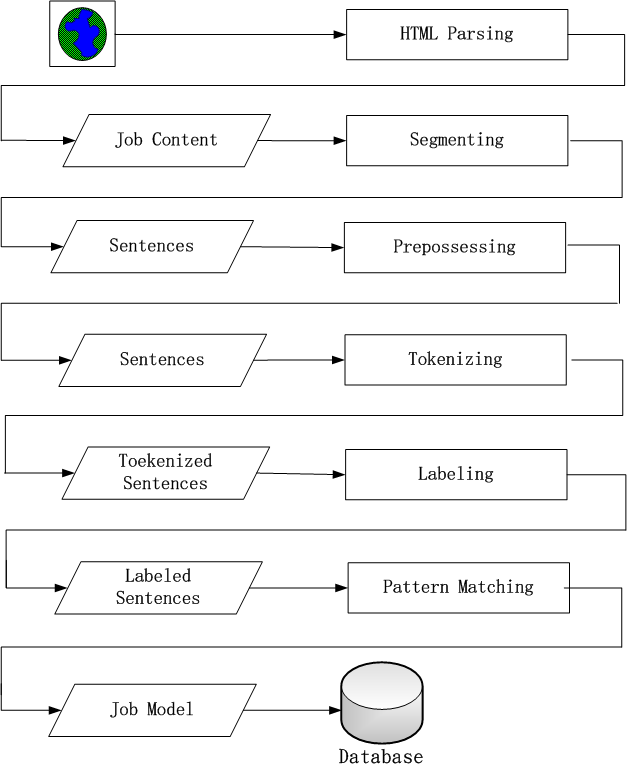
\includegraphics[scale=0.4]{images/pipeline2.png}
  \caption{Job Description Process Pipeline}
  \label{fig:Pipeline}
\end{figure}

\section{Semantic Labeling}

In this section, we will introduce why and how we add two layers of label to the tokenized sentences. In natural language, one concept always have some different expressions. For example, the simple concept bachelor's degree,  has several expressions in job descriptions, e.g. B.S., BA/BS, 4 years degree, and so on. The Table \ref{tab:multispelling} shows the words that if followed with word ``degree'' have the semantic value of ``bachelor's degree''.

\begin{table}[ht]
\caption{All words have meaning bachelors } % title of Table
\centering % used for centering table
\begin{tabular}{  | p{15cm} |  }
 \hline
 "Baccalaureate","bachelors", "bachelor" ,"B.S.", "B.S","BS","BA","BA/BS", "BABS", "BSBA", "B.A." ,"4-year","4-year", "4 year", "four year","college","Undergraduate" , "University" \\
  \hline
\end{tabular}
\label{tab:multispelling} % is used to refer this table in the text\section{Pipeline of Information Extraction}
\end{table}

The regular expression over tokens will transfer a patten to a Finite-State Transducer(FST), and every token of the pattern will be transferred to an edge of FST. If we use all the expressions of a semantic value to create a pattern, the pattern will be very large, and there are too many states in the FST. For example, if we use some words in Table~\ref{tab:multispelling} to create the pattern of semantic value ``bachelor's degree'', the pattern will like below:

$$ (~Baccalaureate~\mid~bachelors~\mid~bachelor~~\mid~B.S~\mid~BS~\mid~BA~)~~degree $$

If all words in Table~\ref{tab:multispelling} are added to the pattern, the FST will have too many edges, and the matching process will be very slow because of the problem of combinatorial explosion.

To resolve this problem, we proposed an approach to use the patterns match the labels of the tokens, not the the original text. Because in the system, we don't care what the words the sentences really use, but want to extract the semantic value of the tokens which match the pattern. The details of the approach is described below:

At first, we created two dictionaries, which are used to labeling the tokens. In the first dictionary, the keys are the tokens, like words in Table~\ref{tab:multispelling}, and the values are the symbols for semantic values, like ``BS-LEVEL'' for ``bachelor's degree'', or ``MS-LEVEL'' for ``master's degree''. In the second dictionary, the keys are semantic values, which are the values of first dictionary. The values of the the second dictionary are the ontology hypernym of their keys, like keys ``BS-LEVEL'' and  ``MS-LEVEL'' both have value ``DE-LEVEL'', which means that bachelor's degree and master's degree are both one kind of degree level.

With the two dictionaries, we can labeling the tokens with two layers. In the first layer, we labeled the tokens with its semantic values, which are the values that we want to extract from the sentence. In the second layer, the labels, which will be matched with patterns, are the ontology hypernyms of the labels in first layer. Table~\ref{tab:labeldsent} shows how the sentence ``Bachelors  degree  in computer science or information systems. '' is labeled.

\begin{table}[ht]
\caption{Labeled sentence } % title of Table
\centering % used for centering table
\begin{tabular}{  | c | c | c | c | c |c | c |c | c | c |  }
 \hline
 layer 2 & DE-LEVEL   & DEGREE & IN & MAJOR            & OR & MAJOR  &.  \\
 \hline
 layer 1 &  BS-LEVEL   & DEGREE & IN & MAJOR-CS         & OR & MAJOR-INFO & .      \\
 \hline
   words & bachelors   & degree & in & computer science & or & information systems & .     \\
  \hline
\end{tabular}
\label{tab:labeldsent} % is used to refer this table in the text\section{Pipeline of Information Extraction}
\end{table}

The pattern ``DE-LEVEL DEGREE  IN   MAJOR  OR  MAJOR ''  matches the sentence above, and the output of the sentence is ``BS-LEVEL'' for bachelor's degree. In the system most patterns match the labels in second layer. With this approach, the states in the pattern will be minimized.

\section{Pattern Matching}

As we explained in last section, we used some patterns over labels in second layer to match the sentences. Some patterns used to match degree phases are in Table ~\ref{tab:patterns}. The patterns looks like regular expression, but they use tokens as the basic units.

\begin{table}[ht]
\small
\caption{Patterns match degree} % title of Table
\centering % used for centering table
\begin{tabular}{  | l  |  }
 \hline
 DE-LEVEL,  DE-LEVEL, OR  DE-LEVEL DEGREE   \\
 DE-LEVEL DEGREE ( IN  $\vert$  OF ) DT MAJOR   \\
 MAJOR-DEGREE  ,  MAJOR-DEGREE OR MAJOR \\
 DE-LEVEL (, DE-LEVEL)* (OR DE-LEVEL)? BE? PERFER-VBD   \\
 \hline
\end{tabular}
\label{tab:patterns} % is used to refer this table in the text\section{Pipeline of Information Extraction}
\end{table}

To matching the labels in sentences, we proposed a library that support matching pattern over tokens. The difference between this library and traditional regular expression is that the basic unit to be matched is token, not character. In the library, a matcher could be a token to be matched, and also could be composition of other matchers. The library supports syntax used in traditional regular expression over string, we list the syntax that the library supports in Table~\ref{tab:matchers}. The first column is the names of the matchers, the second column is the explanation of the function of the matchers, and third column is the their counter part syntaxes of traditional regular expression. The RegexMatcher in library has a regular expression that matches any token matching the regular expression. We give examples of the syntax of these matchers in Table \ref{tab:matchers_example}.

\begin{table}[ht]
\caption{Matcher Class } % title of Table
\centering % used for centering table
\begin{tabular}{  | l | l | l |  }
 \hline
 Matcher Name        &  Function                                 & Counter Part of regex    \\
 \hline
 UnitMatcher       &  token is matches the it                  & character  in regex       \\
 \hline
 SequenceMatcher   &  A list of Matcher                        & sequence of characters       \\
  \hline
 QuestionMatcher   &  One or more of the preceding token       & ?       \\
  \hline
 StarMatcher       &  Zero or more of the preceding token      & *       \\
  \hline
 PlusMatcher       &  Zero or one of the preceding token       & +       \\
  \hline
 DotMatcher        &  Any token                                & .      \\
  \hline
 RegexMatcher      &  Any token matches the regular expression               &        \\
  \hline
\end{tabular}
\label{tab:matchers} % is used to refer this table in the text\section{Pipeline of Information Extraction}
\end{table}



\begin{table}[ht]
\caption{Matcher Class } % title of Table
\centering % used for centering table
\begin{tabular}{  | l |  l |  }
 \hline
 Matcher Name          & Example    \\
 \hline
 UnitMatcher         & DEGREE       \\
 \hline
 SequenceMatcher     & DE-LEVEL DEGREE       \\
  \hline
 QuestionMatcher     & DE-LEVEL (OR DE-LEVEL)?  DEGREE       \\
  \hline
 StarMatcher         & DE-LEVEL (, DE-LEVEL)*  DEGREE       \\
  \hline
 PlusMatcher         & DEGREE IN MAJOR +      \\
  \hline
 DotMatcher          & HAS . DEGREE      \\
  \hline
 RegexMatcher        & r``d-d'' years  \\
  \hline

\end{tabular}
\label{tab:matchers_example} % is used to refer this table in the text\section{Pipeline of Information Extraction}
\end{table}


\section{Regular Expression Over Tokens}

In last section we generally introduced how we use the library of regular expression over tokens to match the sentences. In this section we will introduce more details of this library, like its advantages and implementation details.

\subsection{Finite-State Transducer}
Finite-State Transducer~\cite{roche1997finite} is used as a tool to match patterns and extract information for more than 20 years. This approach have been demonstrated very effective in extracting information from text like CIRCUS~\cite{lehnert1991university} and FASTUS~\cite{hobbs199713}.  In the widely used NLP toolkit GATE~\cite{cunningham2002framework}, the semantic tagger JAPE (Java Annotations Pattern Engine) could describe patterns that are used to match and annotate tokens. JAPE adopts a version of CPSL (Common Pattern  Specification Language)~\cite{appelt1998common}, which provides FST over annotations. Chang et al. presented cascaded regular expressions over tokens~\cite{chang2014tokensregex}, which proposed a cascaded pattern matching tool over token sequences.

After studying these tools, we found most of them are powerful, complex, but not very flexible. One reason is that developers need to learn some DSLs like CPSL, and the other is  integrating the pattern matching tool into the system need extra efforts. So here we proposed a more flexible and lightweight FST framework, which can do regular expression matching over labeled tokens. We give the definition of Finite-State Transducer here. A Finite-State Transducer is a 6-tuple $(\Sigma_1, \Sigma_2, Q, i, F, E)$ where:
\begin{itemize}
  \item $\Sigma_1$ is a finite alphabet, called the input alphabet.
  \item $\Sigma_2$ is a finite alphabet, called the output alphabet.
  \item Q is a finite set of states.
  \item $i \in Q$ is the initial state.
  \item $F \subset Q$ is the set of final states.
  \item $E \subset  Q  \times \Sigma_1^* \times \Sigma_2^* \times Q$ is the set of edges.
\end{itemize}


For example, the FST $T_{d3} = \left(     \{ 0, 1 \} ,  \{ 0, 1 \} , \{ 0, 1 , 2 \} ,  E_{d3} \right ) $ where $E_{d3} = $ \{ ( 0, 0, 0, 0 ),   ( 0, 1, 0, 1 ), ( 1, 0, 0, 2 ), ( 1, 1, 1, 0 ), ( 2, 1, 1, 2 ), ( 2, 0, 1, 1 ) \}  is shown in Figure~\ref{fig:fst}.


\begin{figure}[htbp]
  \centering
  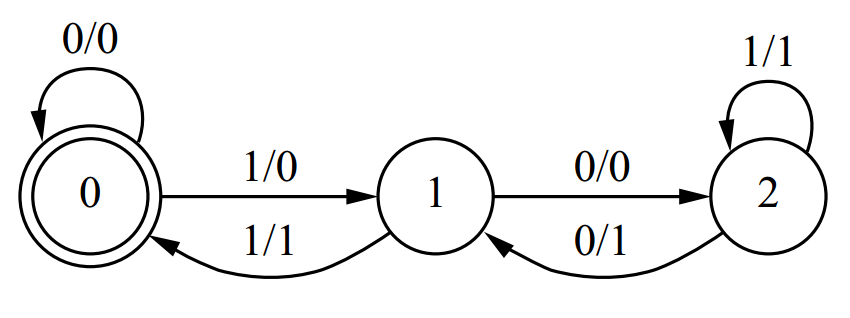
\includegraphics[scale=0.5]{images/fst.png}
  \caption{Zero or one NFA}
  \label{fig:fst}
\end{figure}


\subsection{Flexibility of the library}
The framework supports three styles to create patterns, regular expression style., operator style and  object style. The flexibility of second and third style is that developers could create their own matcher class to extend the feature of the library. We use examples to show how the three styles works. The most common style is defining pattern expression in a string, which is much like traditional regular expression.

\begin{framed}
\small
\noindent
The pattern is:  DE-LEVEL DEGREE ( IN  $\vert$  OF ) DT? MAJOR \\
The code is: \\
seqMatcher =parser.parse("DE-LEVEL DEGREE ( IN  $\vert$  OF ) DT? MAJOR")

\end{framed}

The second style is using algebra operator to connect matchers, as follows:
\begin{framed}
\small
\noindent
The pattern is:  "DE-LEVEL DEGREE (IN $\vert$ OF) MAJOR" \\
The code is: \\
seqMatcher =  UnitMatcher("DE-LEVEL") +  UnitMatcher("DEGREE") + \\
\hspace{3cm} ( UnitMatcher("IN") $\vert$ UnitMatcher("OF" ) ) + UnitMatcher("MAJOR")

\end{framed}

We also could create complex matcher in programming style, which is like we creating and using some objects when programming, as follows:

\begin{framed}
\small
\noindent
The pattern is:  "DE-LEVEL DEGREE (IN $\vert$ OF) MAJOR" \\
The code is: \\
matcher1 = UnitMatcher("DE-LEVEL") \\
matcher2 = UnitMatcher("DEGREE")  \\
matcher3 = UnitMatcher("IN")   \\
matcher4 = UnitMatcher("OF")   \\
matcher5 = UnitMatcher("MAJOR")  \\
matcher6 = AlternateMatcher([matcher3,matcher4])   \\
seqMatcher = SeqMatcher([matcher1, matcher2, matcher6, matcher5])

\end{framed}

The flexibility of the tool also comes from that developers could determine which layer of the array should be matched, the original text or labels in the first or second layer. Developers can assign lambda expressions to the matcher's catching function, which defines how to get the matching input, and out function, which defines what should be outputed. For example,  the labeled sentence is a sequence of arrays, each array includes the original text token and its labels in the other two layers, which is shown in table~\ref{tab:labeldsent}. To match the labeled sentence, we set the lambda expression for catching function to ``lambda x:x[2]'', and the out function to ``lambda x:x[1]'', which make the matcher match the label in second layer, and output the the value of semantic value in the first layer.


\subsection{Implementation of FST Library}

Regular expressions can be converted to automata \cite{aho1992foundations}, and FST is also an automata. To convert a regular expression over token to a FST we need two steps: The first is parsing the expression to a tree of matchers, the second is transfer the tree of matchers to the FST.

We use PLY(Python Lex-Yacc) as the grammar parser, which is a pure-Python implementation of the popular compiler construction tools lex and yacc. We defined  syntaxes of regular expression over token in the parser, which can parse the token regular expression to the tree structure of matchers.

We use the algorithm proposed by Thompson and Ken\cite{thompson1968programming} to construct the FST from the tree of matchers. Each matcher is a partial Nondeterministic Finite Automaton (NFA), which have one or more dangling arrows, pointing to nothing. We build the whole NFA by connecting the arrows of the partial NFAs. Different operator will have different structures of NFA, which is shown below:

The NFAs for matching single token is shown in Figure \ref{fig:nfa_single}.

\begin{figure}[htbp]
  \centering
  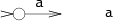
\includegraphics[scale=1]{images/single_token.png}
  \caption{Single Token NFA}
  \label{fig:nfa_single}
\end{figure}

The NFA for the concatenation $e_1e_2$ connects the final arrow of the $e_1$ machine to the start of the $e_2$ machine, which is shown in Figure \ref{fig:nfa_cocat}.

\begin{figure}[htbp]
  \centering
  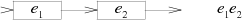
\includegraphics[scale=1]{images/concatenation_tokens.png}
  \caption{Concatenation NFA}
  \label{fig:nfa_cocat}
\end{figure}

The NFA for the alternation $e_1\mid e_2$ adds a new start state with a choice of either the $e_1$ machine or the $e_2$ machine, which is shown in Figure \ref{fig:nfa_alternation}.


\begin{figure}[htbp]
  \centering
  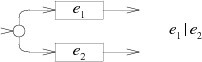
\includegraphics[scale=1]{images/alternation.png}
  \caption{Alternation NFA}
  \label{fig:nfa_alternation}
\end{figure}

The NFA for e? alternates the e machine with an empty path, which is shown in Figure \ref{fig:nfa_question}.


\begin{figure}[htbp]
  \centering
  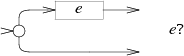
\includegraphics[scale=1]{images/question.png}
  \caption{Zero or one NFA}
  \label{fig:nfa_question}
\end{figure}

The NFA for e* uses the same alternation but loops a matching e machine back to the start, which is shown in Figure \ref{fig:nfa_star}.

\begin{figure}[htbp]
  \centering
  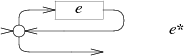
\includegraphics[scale=1]{images/star.png}
  \caption{Zero or more NFA}
  \label{fig:nfa_star}
\end{figure}

The NFA for e+ also creates a loop, but one that requires passing through e at least once, which is shown in Figure \ref{fig:nfa_plus}.

\begin{figure}[htbp]
  \centering
  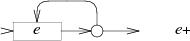
\includegraphics[scale=1]{images/plus.png}
  \caption{One or more NFA}
  \label{fig:nfa_plus}
\end{figure}

With above rules, we can convert the expression ``DL (, DL])*  (or DL)? DEGREE'' to an FST in Figure ~\ref{fig:fst}.

\begin{figure}[htbp]
  \centering
  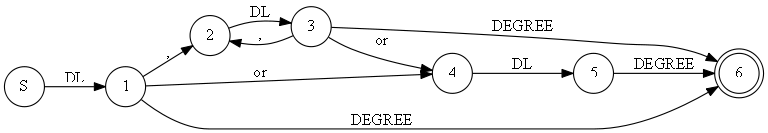
\includegraphics[scale=0.6]{images/test_tokenre2_6.png}
  \caption{Finite Automata Transducers}
  \label{fig:fst}
\end{figure}


